\documentclass[linenumbers, RNAAS, trackchanges]{aastex631}

\usepackage[utf8]{inputenc}
\usepackage{hyperref}           % hrefs
\usepackage{natbib}             % for bibliography
\usepackage{float}              % figure positioning
\usepackage{svg}                % used for SVG images
\usepackage{graphicx}           % used for non-SVG images
\usepackage{amsmath}
\usepackage{parskip}


% Search Query Metadata
\shorttitle{Bessel Functions}
%\shortauthors{Nguyen & Sae}

% Hyperlink setup
\hypersetup{
colorlinks=true,
linkcolor=blue,
urlcolor=blue
}

\begin{document}
\title{Bessel Functions: Theory and Applications}
% [] is for ORCiD
%\correspondingauthor{Main Author}
%\email{author1@email.com, author2@email.com, author3@email.com}
\author{Lily Nguyen}
\affiliation{Department of Physics, The University of Texas at Austin\\
Austin, TX 78712, USA}

\author{Andre Sae}
\affiliation{Department of Physics, The University of Texas at Austin\\
Austin, TX 78712, USA}


% 250 word limit for abstract
\begin{abstract}

We go over three physical scenarios where Bessel Functions are used. The first 
scenario is the infinite square well quantum mechanical wave function in 
spherical coordinates. The second example scenario involves solving the 
temperature equation for thermal diffusion through a material. The final 
example models the vibration along the drum head right after it is struck in 
the middle. 

\end{abstract}

% Use astrothesaurus numbers in place of num
\keywords{word 1 (1) --- word 2 (2) --- word 3 (3) --- word 4 (4)}


\section{Introduction} \label{sec:intro}


For our applications we go over three different physical scenarios where the
conversion of coordinate from cartesian to the coordinate with a radial 
dependency has solutions that contain a Bessel function. The key point between 
each scenario is that the radial dependency in the new coordinate systems 
transforms the second order differential equation whose solution is sinusoidal 
with a damping term or critical damping  into a Bessel function along the radial 
basis. The Bessel function decays to 0 as the input parameter for each physical 
situation radial basis moves toward infinity. However, the physical model does 
resemble the exponential decay pattern found in the physical problems such as a 
spring in fluid simulation.



\section{Data and Observations} \label{sec:data}

\begin{figure}[H]
    \centering
    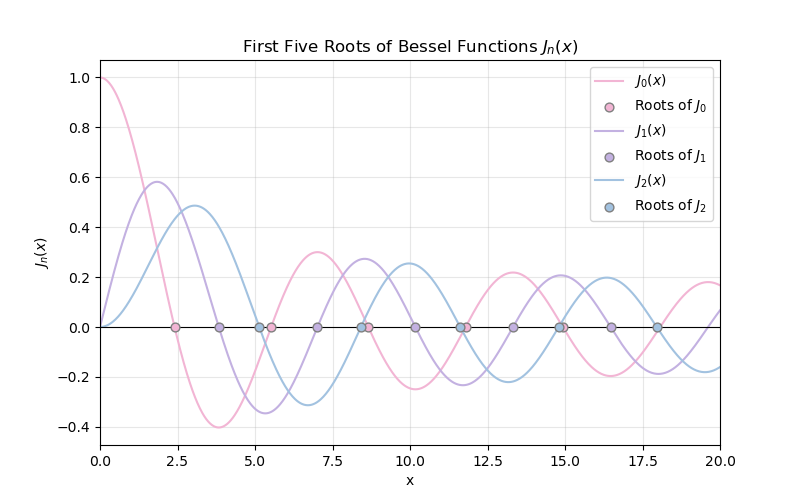
\includegraphics[width=0.70\linewidth]{bessel_roots.png}
    \caption{some caption here}
    \label{fig:bessel_roots}
\end{figure}



\section{Applications} \label{sec:applications}

\subsection{Quantum Mechanics: The Infinite Square Well}
The Bessel function appears in the solution to the wave function of an infinite
square well in spherical coordinates. To solve the quantum mechanics problem, we
define a potential well:

\begin{equation}
    V(x)=
    \begin{cases}
        0, &\text{if }r < a\\
        \infty, &\text{if }r\geq a
    \end{cases}
\end{equation}

The Hamiltonian operator $\hat{H}$ and energy operator $\hat{E}$ must also be
defined to compute the wavefunction. The $n$ and $i$ are quantum numbers where $n$
is the principle quantum number and $I$ is the angular momentum quantum number where
both span the integer range from zero to infinity. $\hbar$ is Planck's constant, $m$
is the mass of the particle, $r$ is the radius, and $R_{n,l}$ is the wavefunction in
the radial basis.

\begin{equation}
    \hat{H}=\frac{-\hbar ^2}{2m}\left(\frac{\partial}{\partial r^2} + \frac{2}{r} \frac{\partial}{\partial r} - \frac{l(l+1)}{r^2}\right) +V(r)
\end{equation}

\begin{equation}
    \hat{H}\psi-E\psi=\hat{H}R_{n,l}-ER_{n,l}=0
\end{equation}

\noindent Applying the Hamiltonial operator on the wavefunction gives us the
spherical Bessel function in differential form, which looks similar to the
origianl Bessel function in differential form:

\begin{equation}
    r^2\frac{\partial R_{n,l}}{partial r^2} + 2r\frac{\partial R_{n,l}}{\partial r} +(k^2r^2-l(l+1))R_{n,l}=0
\end{equation}

\noindent To obtain a solution, we impose a boundary condition $j_l(k_{n,l}a)=0$ at the
bounds of the well. This quantizes our solution by setting a discrete energy
level $E_{n,l}=\frac{\hbar^2k_{n,l}^2}{2ma^2}$ where the solution exists. Hence,
we are left with a radial solution to the wave equation containing the original
Bessel Function:

\begin{equation}
    R_{n,l}=Aj_l(k_{n,l}r)
\end{equation}

\noindent where $j_l(k_{n,l},r)=\sqrt{\frac{\pi}{2kr}}J_{l+\frac{1}{2}}(k_{n,l}R)$.

\subsection{Thermal Diffusion}

We define the heat equation propagating through a two-dimensional surface in
the radial direction. $T$ is the temperature, $t$ is the time, $r$ is the radius,
$k$ is the material conductivity, $\rho$ is the density of the material, and $c_p$
is the specific heat capacity.

\begin{align}
    \frac{\partial T}{\partial t}&=\alpha\nabla^2T\\
    &=\alpha\left(\frac{1}{r} \frac{\partial T}{\partial r} + \frac{\partial^2 T}{\partial r^2}\right)
\end{align}

\noindent where $\alpha=\frac{k}{\rho c_p}$.

To solve this equation, we use separation of variables to split the 
differential equation into two separate differential equations and assume
that one takes the form $T(r,t)=X(r)\theta(t)$. The first equation takes the
form of exponential decay over time:

\begin{equation}
    \frac{d\theta}{dt}+\lambda^2\alpha\theta=0
\end{equation}

\noindent whereas the second equation is the Bessel function of the zeroth-order
since $\alpha=0$:

\begin{equation}
    \frac{d^2X}{dr^2}+\frac{1}{r}\frac{X}{r}+\lambda^2X=0.
\end{equation}

We set a boundary condition of $T(r,t)=T_1$, where $R$ is the radius of the circle,
$t$ is time with $t>0$, and $T_1$ is a constant real value. The initial condition for
the radial space is defined as $T(r,0)=T_2$, where $T_2$ is a constant real value.

\begin{equation}
    T^*=\frac{T(r,t)-T(R,t)}{T(r,0)-T(R,t)}=2\sum_{n=0}^\infty e^{-\beta_{n}^2}
\end{equation}

CAN"T READ EQUATION GO LOOK IN PAPER

\noindent We define temperature as a unitless quantity $T^*$. 

\subsection{Drum Wave Propagation}

Drum wave propagation is similar to thermal diffusion regarding classical wave 
mechanics and quantum mechanics through the quantization of boundary conditions.
We define a wavefunction for the propagation across a drum surface where $\sigma$
is the surface mass density of the membrane and $S$ is the surface tension
across the membrane:

\begin{equation}
    \frac{\partial^2z}{\partial t^2}=c^2\nabla^2z
\end{equation}

\noindent where $c^2=\frac{\sigma^2}{S}$.

The first boundary condition is $z(R_f,t)=0$. The displacement ...

\section{Results} \label{sec:results}



\subsection{Acknowledgements}
We thank Professor Mitra for his guidance and instruction throughout the course,
as well as the teaching assistants for their helpful feedback. We also
acknowledge the Department of Physics for providing an excellent academic foundation 
to support this work. This work was completed as part of the requirements for 
C S 323E: Elements of Scientific Computing at the University of Texas at Austin.

\newpage
\bibliographystyle{aasjournal}
\bibliography{refs}

\end{document}